\documentclass{article}

%\usepackage{corl_2023} % Use this for the initial submission.
\usepackage[final]{corl_2023} % Uncomment for the camera-ready ``final'' version.
%\usepackage[preprint]{corl_2023} % Uncomment for pre-prints (e.g., arxiv); This is like ``final'', but will remove the CORL footnote.

\usepackage{graphicx}
\usepackage{amssymb}
\usepackage{amsmath}
\usepackage{listings}
\usepackage{subcaption}
\usepackage{latexsym}
\usepackage{amsthm}
\usepackage{natbib}
\usepackage{listings}
\usepackage{hyperref} 

\title{Exercise 2 - Robot Learning Course}

% The \author macro works with any number of authors. There are two
% commands used to separate the names and addresses of multiple
% authors: \And and \AND.
%
% Using \And between authors leaves it to LaTeX to determine where to
% break the lines. Using \AND forces a line break at that point. So,
% if LaTeX puts 3 of 4 authors names on the first line, and the last
% on the second line, try using \AND instead of \And before the third
% author name.

% NOTE: authors will be visible only in the camera-ready and preprint versions (i.e., when using the option 'final' or 'preprint'). 
% 	For the initial submission the authors will be anonymized.

\author{
  Andrea Ongaro\\
	Computer Engineering\\
	Politecnico di Torino, Italy\\
	\texttt{s329706@studenti.polito.it} \\
  %% examples of more authors
  %% \And
  %% Coauthor \\
  %% Affiliation \\
  %% Address \\
  %% \texttt{email} \\
  %% \AND
  %% Coauthor \\
  %% Affiliation \\
  %% Address \\
  %% \texttt{email} \\
  %% \And
  %% Coauthor \\
  %% Affiliation \\
  %% Address \\
  %% \texttt{email} \\
  %% \And
  %% Coauthor \\
  %% Affiliation \\
  %% Address \\
  %% \texttt{email} \\
}


\begin{document}
\maketitle

%===============================================================================

\begin{abstract}
This article is the second in a series of three for the Reinforcement Learning laboratory course at Politecnico di Torino. In this report, it's explored the potential of Q-learning within the OpenAI Gym environment, focusing on the CartPole problem. The analysis includes experiments with different epsilon values and various Q-table initialization strategies. 

\end{abstract}

% Two or three meaningful keywords should be added here
\keywords{Reinforcement Learning, Robots, AI} 

%===============================================================================

\section{Introduction}
\subsection{The system - CartPole-v0}
CartPole-v0 system from OpenAI is part of the classic control environment. The starting code it's been provided by \href{https://www.polito.it/personale?p=andrea.protopapa}{Andrea Protopapa} in the course of Reinforcement Learning. Information about this system is sourced from the official documentation \cite{Cart_pole} and its GitHub repository. Below is the definition provided by the authors for CartPole-v0\\ \\
\textit{This environment corresponds to the version of the cart-pole problem described by Barto, Sutton, and Anderson in “Neuronlike Adaptive Elements That Can Solve Difficult Learning Control Problem”. A pole is attached by an un-actuated joint to a cart, which moves along a frictionless track. The pendulum is placed upright on the cart and the goal is to balance the pole by applying forces in the left and right direction on the cart.\citep{Cart_pole}}

\begin{figure}[h]
	\centering
	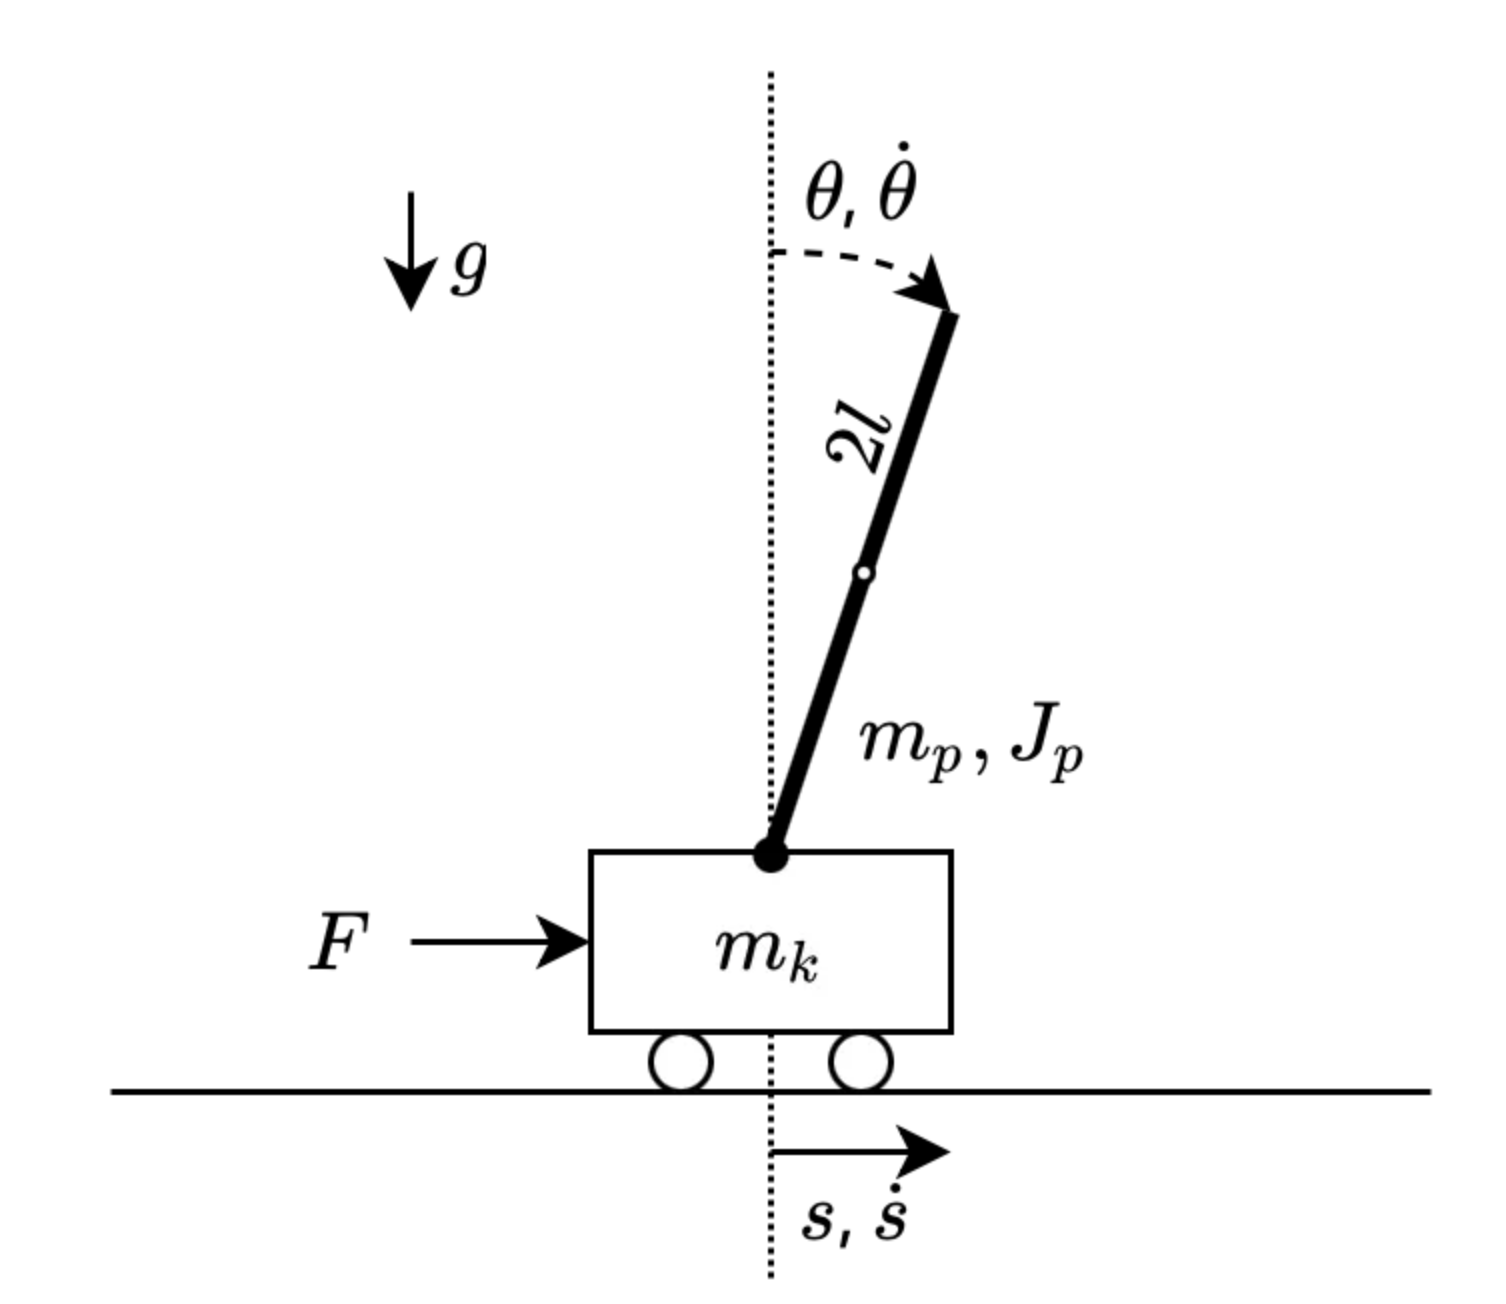
\includegraphics[width=0.5\linewidth]{../data/images/cart.png}
	\caption{Graphical explation about the whole system}
	\label{fig:plot1}
\end{figure}

\newpage

The observation is a four element vector: 
\begin{figure}[h]
	\centering
	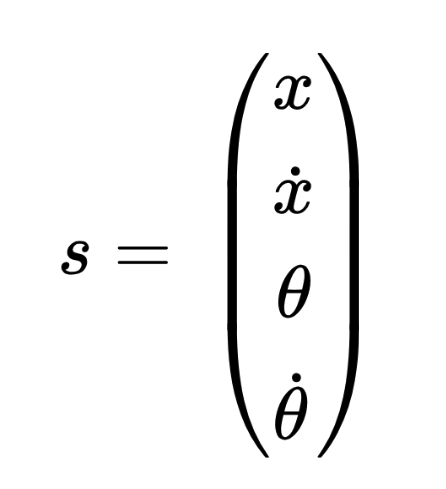
\includegraphics[width=0.2\linewidth]{../data/images/vector.png}
	\caption{Observation vector}
	\label{fig:plot1}
\end{figure}

where 
\begin{itemize}
	\item $x$: the position of the cart
	\item $\dot{x}$: the velocity, 
	\item $\theta$:  the angle of the pole
	\item $\dot{\theta}$: the angular velocity of the pole., 	
\end{itemize}

\subsection{Q-Learning}
Q-learning is a model-free reinforcement learning algorithm that relies on trial-and-error methods. Unlike model-based approaches, it does not construct an internal model of the environment or explicitly use a Markov Decision Process. Instead, the agent learns directly from the outcomes of its actions by interacting with the environment.

Initially, the agent is aware of the set of possible states and actions within the environment but has no knowledge of how these states transition or what rewards they yield. Through exploration, the agent gradually discovers state transitions and rewards, enabling it to improve its policy over time.

\begin{figure}[h]
	\centering
	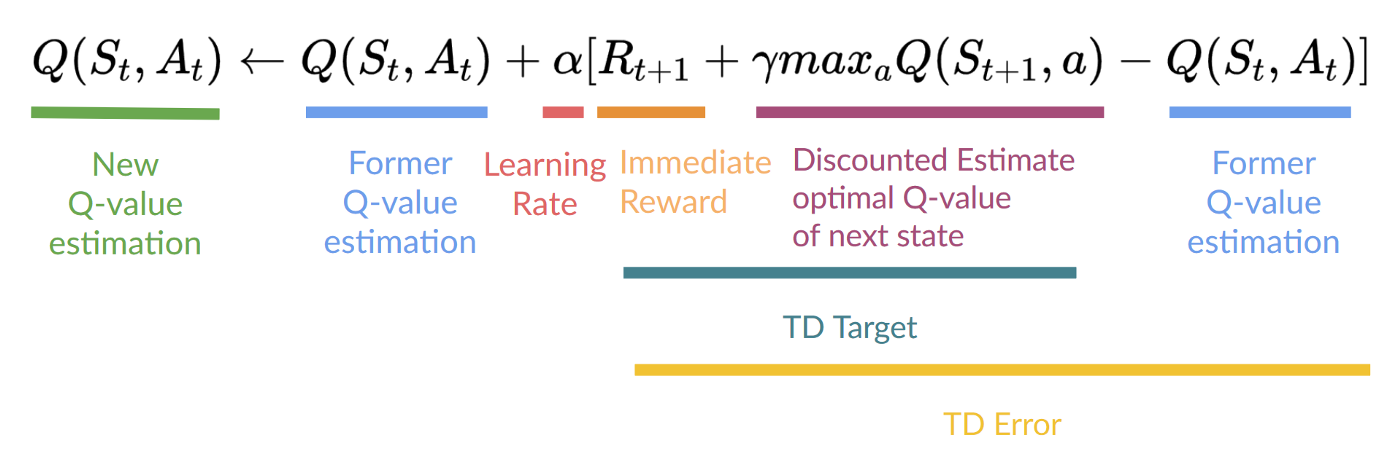
\includegraphics[width=0.5\linewidth]{../data/images/Q-learning-8.png}
	\caption{Q-value estimation}
	\label{fig:q_learning}
\end{figure}

\subsubsection{Exploration vs. Exploitation Tradeoff}
An agent interacts with its environment by taking actions and observing the outcomes. During this process, the agent has a set of actions to choose from. Some actions may have been taken previously, allowing the agent to predict their outcomes, while others remain unexplored and unpredictable.

This balance between leveraging known actions and exploring new ones is called the \textbf{exploration-exploitation trade-off.}
\begin{itemize}
	\item When the agent \textbf{explores}, it experiments with unfamiliar actions, expanding its knowledge and potentially improving long-term rewards.
	\item Conversely, when the agent \textbf{exploits}, it chooses actions based on what it already knows to maximize immediate rewards, even if this behavior might be suboptimal in the long run.
\end{itemize}

A \textbf{trade-off is necessary} since the agent cannot explore and exploit simultaneously . At the start of training, the agent has no knowledge about the consequences of its actions, so sufficient initial exploration is crucial. This allows the agent to identify actions that yield higher rewards. However, relying solely on exploitation can be risky, as it prevents the agent from discovering better strategies or optimal behaviors.

\subsubsection{$\epsilon$ greedy}
In Q-learning, the agent selects an action based on the reward it expects to receive, aiming to maximize the cumulative reward over time. It always chooses the action that leads to the highest estimated reward for the given state, which ensures that it generates the maximum possible reward in that state.

On the other hand, the epsilon-greedy strategy introduces a balance between exploitation (using prior knowledge to select the best action) and exploration (trying new actions to potentially discover better options). The agent typically selects the action with the highest estimated reward most of the time but occasionally explores other actions.

The strategy incorporates an exploration factor, denoted by $\epsilon$ (epsilon), which determines the probability of choosing a random action. With a small probability of $\epsilon$, the agent will explore by selecting an action at random, regardless of its current knowledge of action values. The remaining time, with probability 1 - $\epsilon$, the agent exploits its knowledge and chooses the action with the highest Q-value, thus maximizing the expected reward.

\begin{figure}[h]
	\centering
	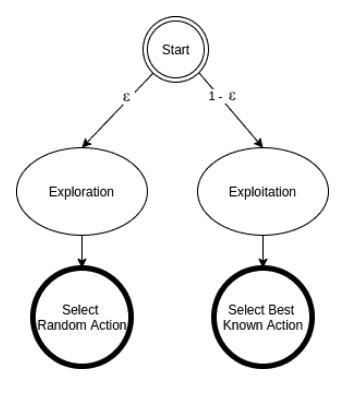
\includegraphics[width=0.3\linewidth]{../data/images/exp_e.png}
	\caption{Exploitation vs Exploration \cite{q_le}}
	\label{fig:expl}
\end{figure}

\subsubsection{GLIE - greedy in limit with infinite exploration}

GLIE (Greedy in the Limit with Infinite Exploration) ensures that each action of a state that is visited often is, in turn, chosen infinitely often (with probabilty of 1) allowing for comprehensive exploration of the environment. Over time, the learning policy converges to a greedy approach with respect to the Q-value function.

%Each action is executed infinitely often in every state that is visited infinitely often;
%In the limit, the learning policy is greedy with respect to the Q-value function with probability 1
% https://users.ece.cmu.edu/~yuejiec/ece18813B_notes/lecture10-online-RL-GLIE.pdf

\subsubsection{Heatmap}
A heatmap can be utilized to analyze the current state of the system under study. The heatmap depicts values for a main variable of interest across two axis variables as a grid of colored squares. The axis variables are divided into ranges like a bar chart or histogram, and each cell’s color indicates the value of the main variable in the corresponding cell range \cite{heatmap}. \\ 

Each cell can represent different states, ranging from high-value regions, which correspond to states where the agent expects to achieve high cumulative rewards (e.g., states near the upright pole position with low velocity and angular velocity), to low-value regions, which represent states likely to lead to termination or failure (e.g., the pole falling or the cart moving out of bounds).

\newpage

\section{Methodology}

\subsection{Fixed $\epsilon$ vs GLIE epsilon schedule}
They're been developed three different strategies, two of which will be compared in the following paragraph. The first strategy uses a constant epsilon value of 0.2  ($\epsilon =  0.2$) while the second employs the following formula (Equation \ref{formula:epsilon}) where epsilon decreases to 0.1 after 20.000 episodes. To achieve this, we set the value of b to 2221, which ensures that at the end of the GLIE schedule, epsilon will be approximately equal to $0.09995049727735025$

\centering
\label{formula:epsilon}
$ e_k = b / (b+k) $ 

\flushleft

The reward trends for the two plots reveal distinct patterns. In the first plot (Figure \ref{fig:costant_eps}), there is a rapid initial rise in rewards during the early episodes, indicating steep learning, followed by stabilization around an average of 150-175 with consistent fluctuations. The second plot (Figure  \ref{fig:glie_eps})  also shows a sharp initial rise, but the rewards exhibit greater variability in later episodes and seem to slightly decline after about episode 15,000. 

In terms of variability, the first plot displays more stable reward trends after the initial learning phase, with spikes that are present but not extreme, whereas the second plot contains more pronounced and frequent fluctuations throughout training.

%Speaking about the performance between a fixed epsilon vs. the GLIE epsilon schedule, there is no much difference between them. Overall the second reward \ref{glie_eps} is initially lower but it finally achieve an higher one. 
%Looking at the testing render you can see an improvement compared to the fixed epsilon it happen more times than the first to arrive at the end of the episode succeding in mantaining the pole stable, but it's not perfect anyway.

\begin{figure}[h]
	\centering
	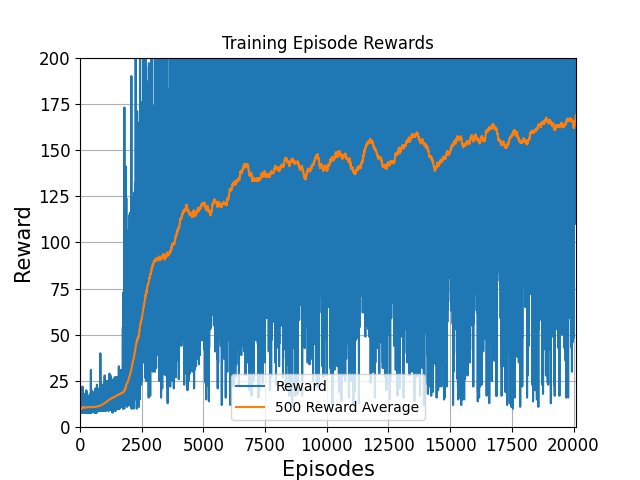
\includegraphics[width=0.5\linewidth]{../data/plot/q_learning_constant_0.2.png}
	\caption{Reward obtained - $\epsilon = 0.2$}
	\label{fig:costant_eps}
\end{figure}

\begin{figure}[h]
	\centering
	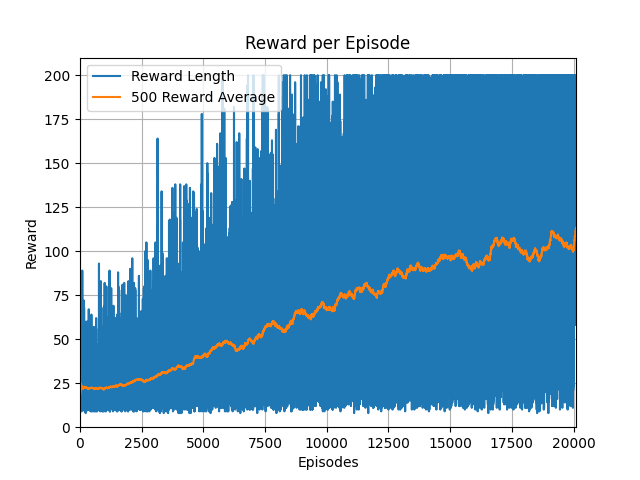
\includegraphics[width=0.5\linewidth]{../data/plot/q_learning_GLIE.png}
	\caption{Reward obtained - Formula \ref{formula:epsilon}}
	\label{fig:glie_eps}
\end{figure}

\subsubsection{Value function}
After computing the associated value function, the heatmap of the computed value function in terms of $ x $ and $\theta$,(the current position of the cart and the pole angle) was generated. To plot this, the values were averaged over $\dot{x} $ and $\dot{\theta} $.

The focus will be on the Q-value heatmap at different stages of the training: before training, after a single episode, after half of the episodes and at full training. The general trend is consistent between the two methodologies. These heatmaps can be found in the data/plots folder for further analysis.


\subsubsection{Before training}
Before training the heatmap is likely flat, with no clear structure. All state-action pairs have equal zero Q -values, meaning  the value function is uniform across states. The agent has no prior knowledge of the environment. See Figure \ref{fig:heatmap_init_costant} and Figure \ref{fig:heatmap_init_glie}.

\begin{figure}[h]
		\centering
		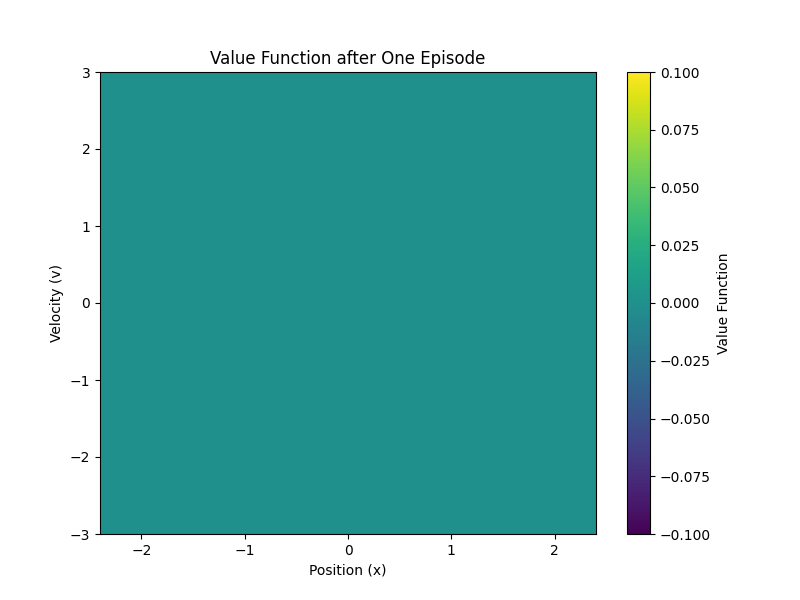
\includegraphics[height=0.28\linewidth]{../data/plot/heatmap_initial_training_constant_0.2.png}
		\caption{Heatmap in the initial state \\ using $\epsilon = 0.2$}
		\label{fig:heatmap_init_costant}
\end{figure}

\begin{figure}[h]
		\centering
		\includegraphics[height=0.28\linewidth]{../data/plot/heatmap_initial_training_glie.png}
		\caption{Heatmap in the initial state \\ using Formula \ref{formula:epsilon}}
		\label{fig:heatmap_init_glie}
\end{figure}

\newpage

\subsubsection{After one episode}
After one episode some regions of the heatmap may begin to show slightly higher values, particularly in states visited during the episode. The updates are sparse and localized around the trajectory the agent followed during the episode. Unvisited states retain their initial values, while the agent updates the Q-values for the specific states and actions it encountered, thereby improving its estimate of $ V(s) $  in those regions.
As a result, most of the state space remains unexplored, leading to minimal structure in the heatmap. 

The second image (Figure \ref{fig:heatmap_costant_init}) shows a wider range of values, suggesting the agent has learned a more diverse set of values across the different positions of the cart while the first one (Figure \ref{fig:heatmap_glie_init}), with a narrower value range, suggests it has learned a more limited set of values after a single episode.

\begin{figure}[h]
	\centering
	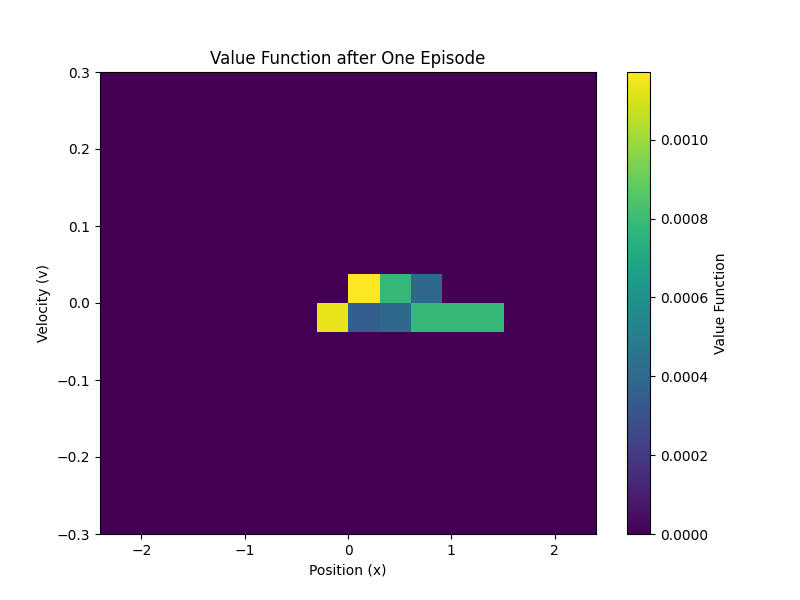
\includegraphics[height=0.28\linewidth]{../data/plot/heatmap_after_one_episode_constant_0.2.png}
	\caption{Heatmap after one single episode \\ using $\epsilon = 0.2$}
	\label{fig:heatmap_costant_init}
\end{figure}

\begin{figure}[h]
	\centering
	\includegraphics[height=0.28\linewidth]{../data/plot/heatmap_after_one_episode_glie.png}
	\caption{Heatmap after one single episode \\ using Formula \ref{formula:epsilon}}
	\label{fig:heatmap_glie_init}
\end{figure}

\newpage
\subsubsection{Half-way training}
The heatmap begins to take shape, revealing a clearer distinction between “good” and “bad” states. Some areas may still appear noisy or less structured, particularly in regions that have been underexplored. (Figure \ref{fig:heatmap_costant_half}
and \ref{fig:heatmap_glie_half})

\begin{figure}[h]
		\centering
		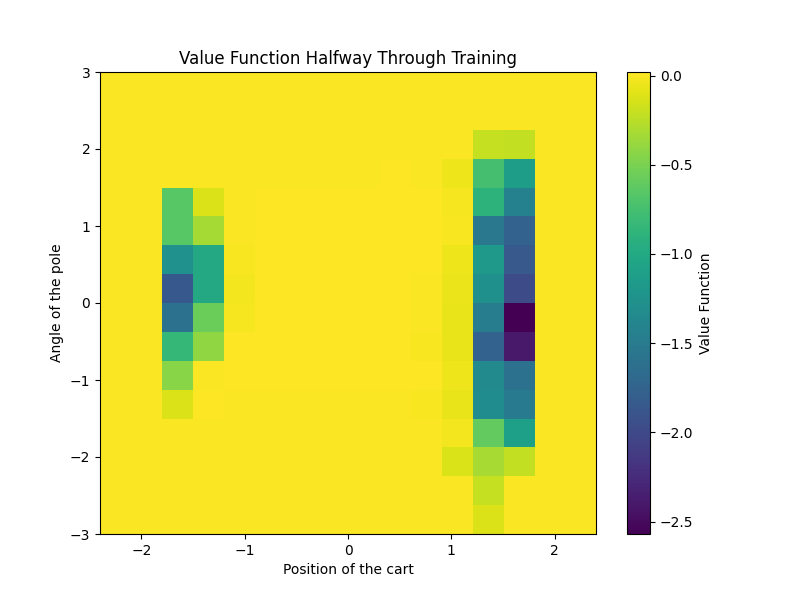
\includegraphics[height=0.28\linewidth]{../data/plot/heatmap_halfway_constant_0.2.png}
		\caption{Halfway Training Heatmap  \\ using $\epsilon = 0.2$}
		\label{fig:heatmap_costant_half}
\end{figure}

\begin{figure}[h]
		\centering
		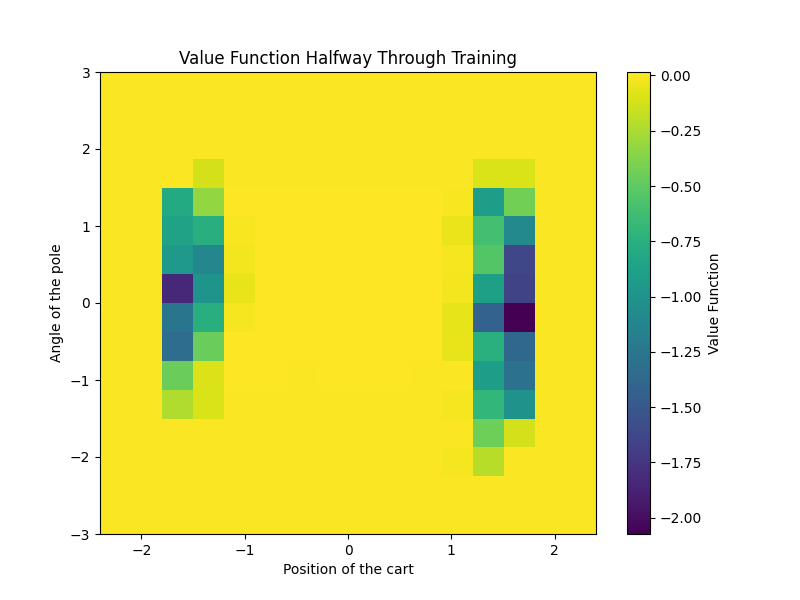
\includegraphics[height=0.28\linewidth]{../data/plot/heatmap_halfway_GLIE.png}
		\caption{Halfway Training Heatmap  \\ using Formula \ref{formula:epsilon}}
		\label{fig:heatmap_glie_half}
\end{figure}

\subsubsection{Full training}
Analyzing  the two full training heatmaps (Figure \ref{fig:heatmap_costant_full} and Figure \ref{fig:heatmap_glie_full}), it is clear that the agent has effectively learned the optimal policy, even if they're slighly different. The heatmaps are smooth and clear, with distinct high-value regions corresponding to optimal solution. 
\begin{figure}[h]
	\centering
	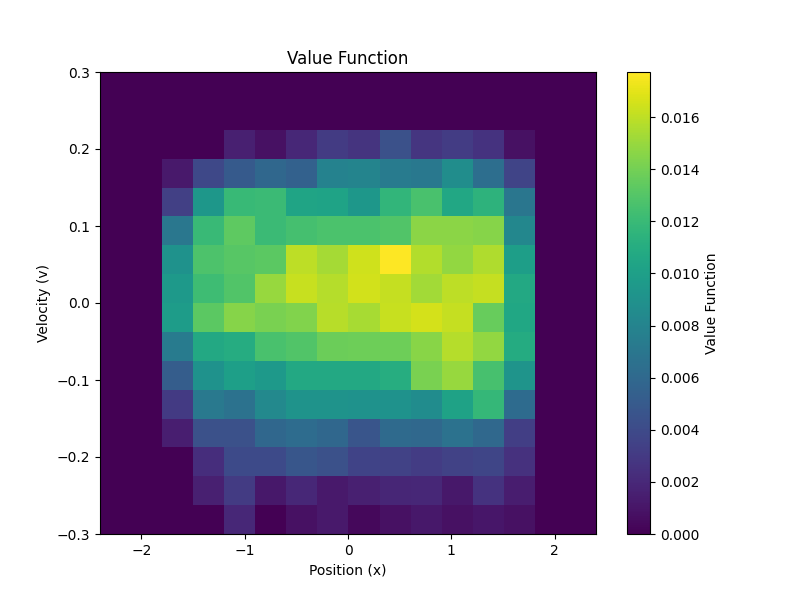
\includegraphics[height=0.28\linewidth]{../data/plot/heatmap_full_training_constant_0.2.png}
	\caption{Heatmap image - $\epsilon = 0.2$}
	\label{fig:heatmap_costant_full}
\end{figure}

\begin{figure}[h]
	\centering
	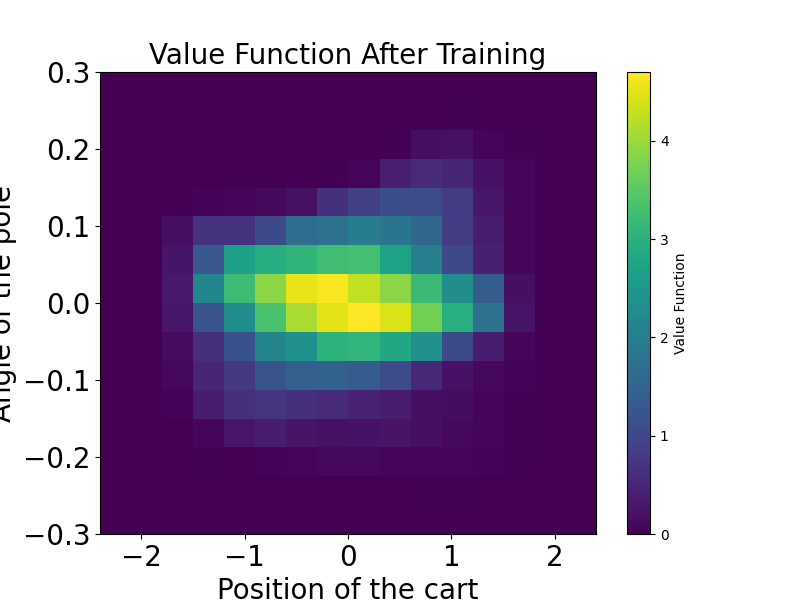
\includegraphics[height=0.28\linewidth]{../data/plot/heatmap_full_training_GLIE.png}
	\caption{Heatmap image - Formula \ref{formula:epsilon}}
	\label{fig:heatmap_glie_full}
\end{figure}


\newpage

\subsection{Epsilon zero}
The final strategy analyzed in this article involves setting epsilon to 0. With epsilon set to 0, there is no exploration, meaning the agent relies solely on its current knowledge without attempting to discover new states or actions. Without exploration, there is no guarantee that the agent can sufficiently learn the environment to identify the optimal policy and it may stuck in \textbf{sub-optimal policy}.\\
In this subsection, the scenario of epsilon equal to zero is examined under two different cases:
\begin{itemize}
	\item keeping the initial Q-function values at zero;
	\item setting the initial Q-function values at 50 for all states and actions;
\end{itemize}

\subsubsection{Comparison}
Initializing the Q-function introduces a certain degree of bias. Initializing Q-values n to 50, the agent assumes it can achieve high rewards from all state-action pairs initially. As a result, convergence becomes slower because the updates to the Q-values take longer to overwrite these inflated initial values.

The second approach proves to be more effective, leading to a better estimation of the Q-function. This improvement stems from the nature of the greedy policy, which consistently selects actions that maximize the cumulative reward for a given state. When the Q-function is initialized to the same value for all state-action pairs, the greedy policy initially has no preference and is forced to randomly select actions. This randomness ensures that the agent begins to estimate the values of the actions it takes for each state.

Then the optimistic initialization encourages exploration. At first, the agent assumes all actions will yield high rewards (+50). However, as actions are taken, the agent receives rewards that are typically lower than this optimistic estimate. This “disappointment” motivates the agent to switch to other actions, resulting in all actions being explored multiple times before the Q-values converge. Consequently, this approach achieves a significant amount of exploration even when the policy remains greedy (i.e., always selecting the current best-known action).

As expected, instead, the first approach fails to discover new actions and results in suboptimal performance (Figure \ref{fig:heatmap_zero} and Figure \ref{fig:reward_zero})

\begin{figure}[h]
		\centering
		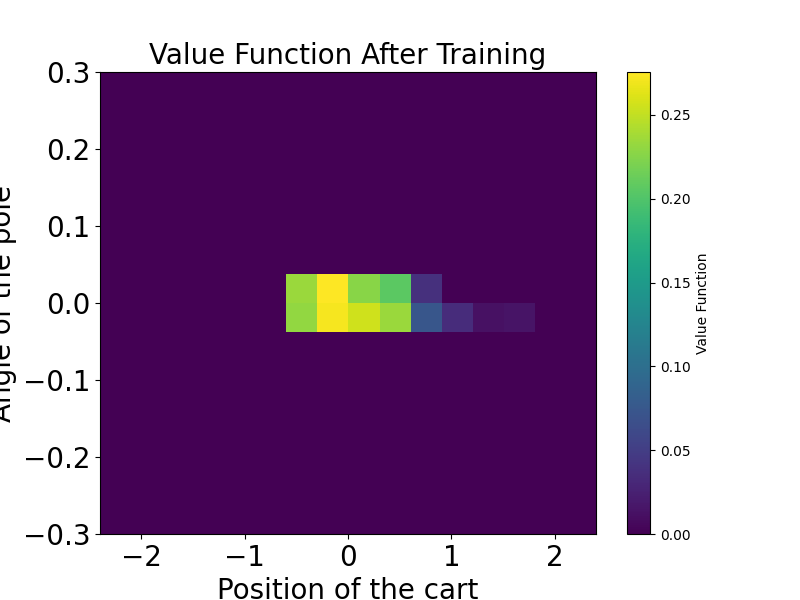
\includegraphics[height=0.28\linewidth]{../data/plot/heatmap_full_training_zero_epsilon.png}
		\caption{Full training Heatmap with $\epsilon = 0$ }
		\label{fig:heatmap_zero}
\end{figure}

\begin{figure}[h]
	\centering
	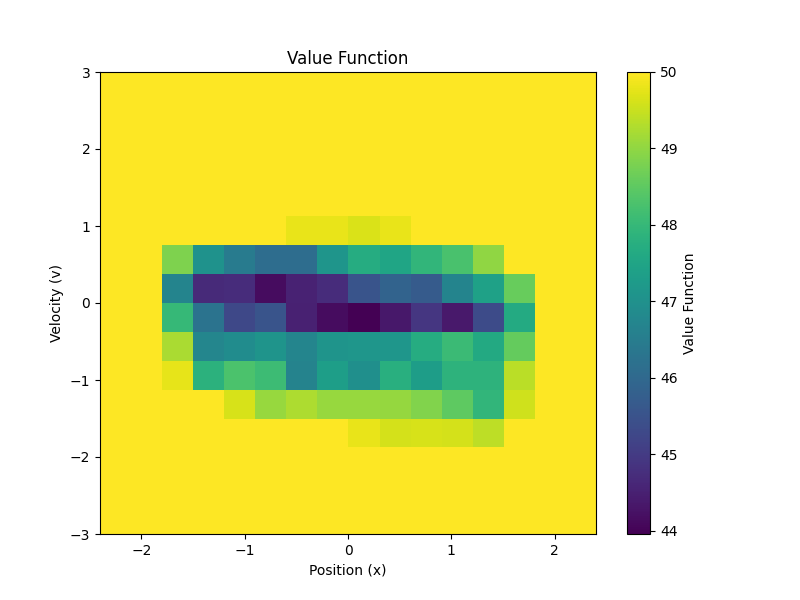
\includegraphics[height=0.28\linewidth]{../data/plot/heatmap_full_training_zero_epsilon_fifty_initial.png}
	\caption{Reward obtained with $\epsilon = 0$ and $Q values = 50$}
	\label{fig:heatmap_zero_fifty}
\end{figure}

\begin{figure}[h]
	\centering
	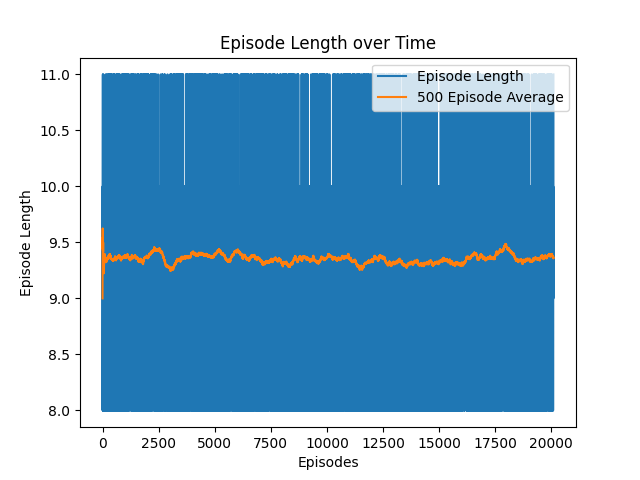
\includegraphics[height=0.28\linewidth]{../data/plot/q_learning_zero_epsilon.png}
	\caption{Full training Heatmap with $\epsilon = 0$ }
	\label{fig:reward_zero}
\end{figure}


\begin{figure}[h]
		\centering
		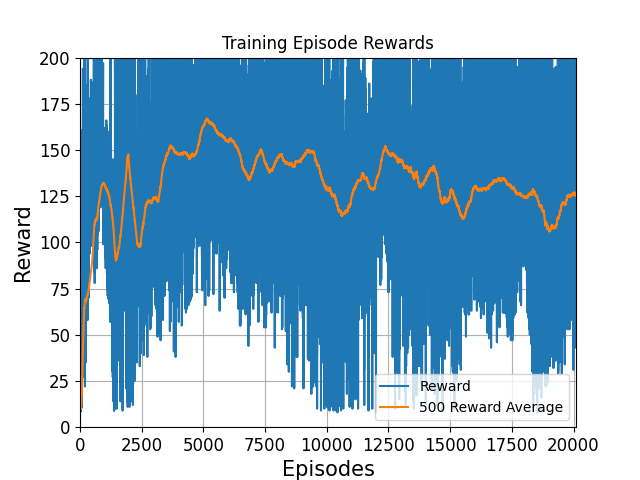
\includegraphics[height=0.28\linewidth]{../data/plot/q_learning_zero_epsilon_fifty_initial.png}
		\caption{Reward obtained with $\epsilon = 0$ and $Q values = 50$}
		\label{fig:reward_zero_fifty}
\end{figure}


\newpage

\section{Q-Learning : Different applications}

\subsection{Continuous state spaces}
Q-learning can be adapted for environments with continuous state spaces, but it requires some modifications because the algorithm inherently relies on a discrete state-action table. A common approaches for continuous state spaces is to use a state discretization, as it's been done in this article. 

It is important to note that discretization can result in a loss of precision and is particularly affected by the “curse of dimensionality”\cite{BELLMAN1958228} in high-dimensional spaces. 

To overcome this problem there is an alternative that involves the use of the function approximators (e.g., neural networks, decision trees, or linear regression) to represent the Q-function Q(s, a) instead of a table. This permits to handles continuous state spaces directly without discretization and scales better to high dimensions and it's the foundation of Deep Q-Learning (DQN), where neural networks approximate $ Q(s, a) $.
 
% Divide the continuous state space into discrete bins (grids).
% Each bin represents a discrete state, and standard Q-learning operates on this discretized state space.
\subsection{Continuous action spaces}
% https://ai.stackexchange.com/questions/12255/can-q-learning-be-used-for-continuous-state-or-action-spaces
% https://www.quora.com/Why-doesn-t-Q-learning-work-with-continuous-action-spaces
The challenge of applying Q-learning to continuous action spaces becomes apparent when examining the TD Target (see Figure \ref{fig:q_learning}). The process of determining the maximum Q-value for the next state becomes increasingly inefficient and less accurate as the size of the action space grows.

In continuous action spaces, where the number of possible actions is infinite, it is impossible to simply scan all actions to identify the one that produces the maximum Q-value. This makes the traditional max operation computationally impractical.

One potential solution is to discretize the action space, reducing it to a finite set of actions. However, this approach can lead to a loss of precision and may not be suitable for all problems.

To address this issue, variants of Q-learning have been developed. These methods not only approximate the Q-value function but also approximate the max operation itself, enabling the algorithm to handle continuous action spaces more effectively.

%===============================================================================

%===============================================================================

%===============================================================================

% no \bibliographystyle is required, since the corl style is automatically used.
\bibliography{example}  % .bib

\end{document}
